\documentclass{article}

\usepackage{tikz}
\usetikzlibrary{shapes.geometric, arrows}

%
% Define the building blocks of the flowchart.
%

\tikzstyle{startstop} = [rectangle, rounded corners, minimum width=3cm, minimum height=1cm,text centered, text width=3cm, draw=black]

\tikzstyle{io} = [trapezium, trapezium left angle=70, trapezium right angle=110, minimum width=3cm, minimum height=1cm, text centered, draw=black, fill=white]

\tikzstyle{process} = [rectangle, minimum width=3cm, minimum height=1cm, text centered, text width=3cm, draw=black, fill=white]

\tikzstyle{decision} = [diamond, minimum width=3cm, minimum height=1cm, text centered, draw=black]

\tikzstyle{arrow} = [thick,->,>=stealth]

%
% Document.
%

\begin{document}

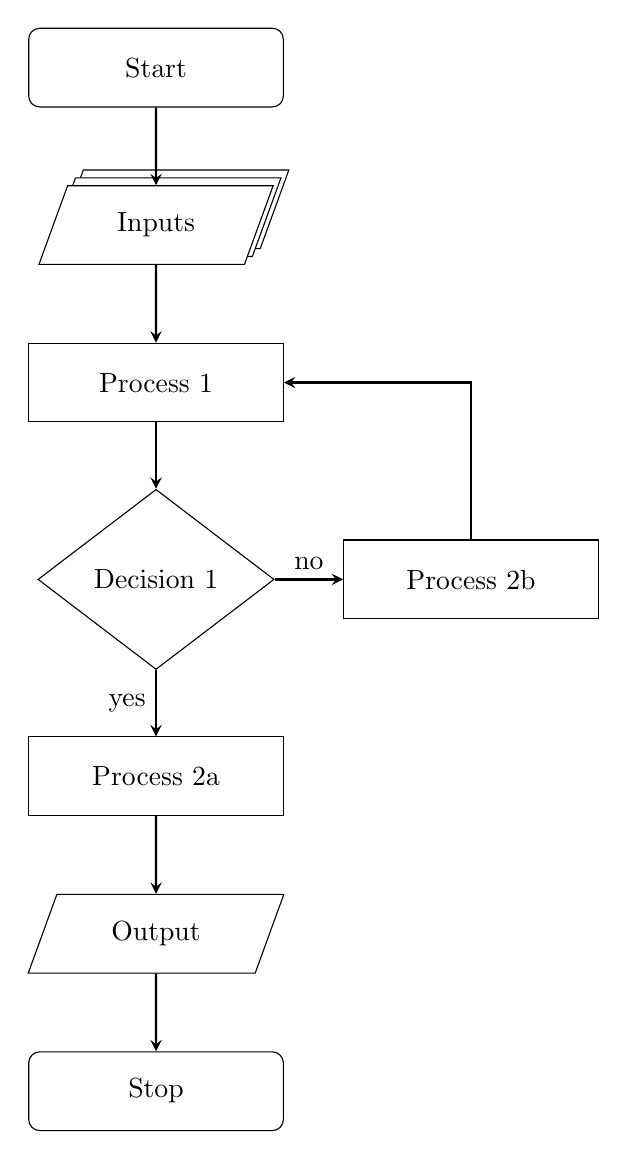
\begin{tikzpicture}[node distance=2cm]

\node (start) [startstop] {Start};
\node () [io, below of=start, yshift=+0.2cm, xshift=+0.2cm] {Inputs};
\node () [io, below of=start, yshift=+0.1cm, xshift=+0.1cm] {Inputs};
\node (in1) [io, below of=start] {Inputs};
\node (pro1) [process, below of=in1] {Process 1};
\node (dec1) [decision, below of=pro1, yshift=-0.5cm] {Decision 1};
\node (pro2a) [process, below of=dec1, yshift=-0.5cm] {Process 2a};
\node (pro2b) [process, right of=dec1, xshift=2cm] {Process 2b};
\node (out1) [io, below of=pro2a] {Output};
\node (stop) [startstop, below of=out1] {Stop};

\draw [arrow] (start) -- (in1);
\draw [arrow] (in1) -- (pro1);
\draw [arrow] (pro1) -- (dec1);
\draw [arrow] (dec1) -- node[anchor=east] {yes} (pro2a);
\draw [arrow] (dec1) -- node[anchor=south] {no} (pro2b);
\draw [arrow] (pro2b) |- (pro1);
\draw [arrow] (pro2a) -- (out1);
\draw [arrow] (out1) -- (stop);

\end{tikzpicture}

\end{document}
